\chapter{Architettura}
\section{Introduzione}
L'architettura di \textit{Login Warrior} è basata sul design pattern architetturale$_G$ \textit{Model-View-Controller}. Il gruppo ha sviluppato un controller per ognuna delle due pagine dell'applicazione, i quali devono gestire le interazioni dell'utente con la \textit{GUI}$_G$.

 Le viste corrispondono alle pagine dell'applicazione e sono quindi due: la pagina home nella quale verrà caricato il dataset e visualizzata la lista dei grafici disponibili, e quella dove verrà effettivamente visualizzato il grafico con relativi filtri e customizzazioni.

 Il modello contiene i dati da visualizzare, che vengono presi dal file \textit{CSV} e convertiti in oggetti di tipo \textit{DataPoint} contenuti nell'oggetto \textit{Dataset}.

 Dato che viene utilizzato il servizio IndexeedDB dei browser, il gruppo ha ritenuto che questo non facesse parte di nessuno dei tre componenti sopra descritti, e quindi ha deciso di separarlo mettendolo in \textit{Services}. È comunque il controller che si occupa di gestirlo.


È stato scelto il design pattern MVC per i seguenti motivi:
\begin{itemize}
  \item Favorisce la separazione tra \textit{business logic} e \textit{presentation logic}, facendo comunicare modello e vista solo attraverso il controller;
  \item Adatto per le applicazioni che prevedono una \textit{GUI} per l'interazione con l'utente.
\end{itemize}
\section{Diagrammi delle classi}
\subsection{Model}
\subsection{View}
\begin{figure}[H]
    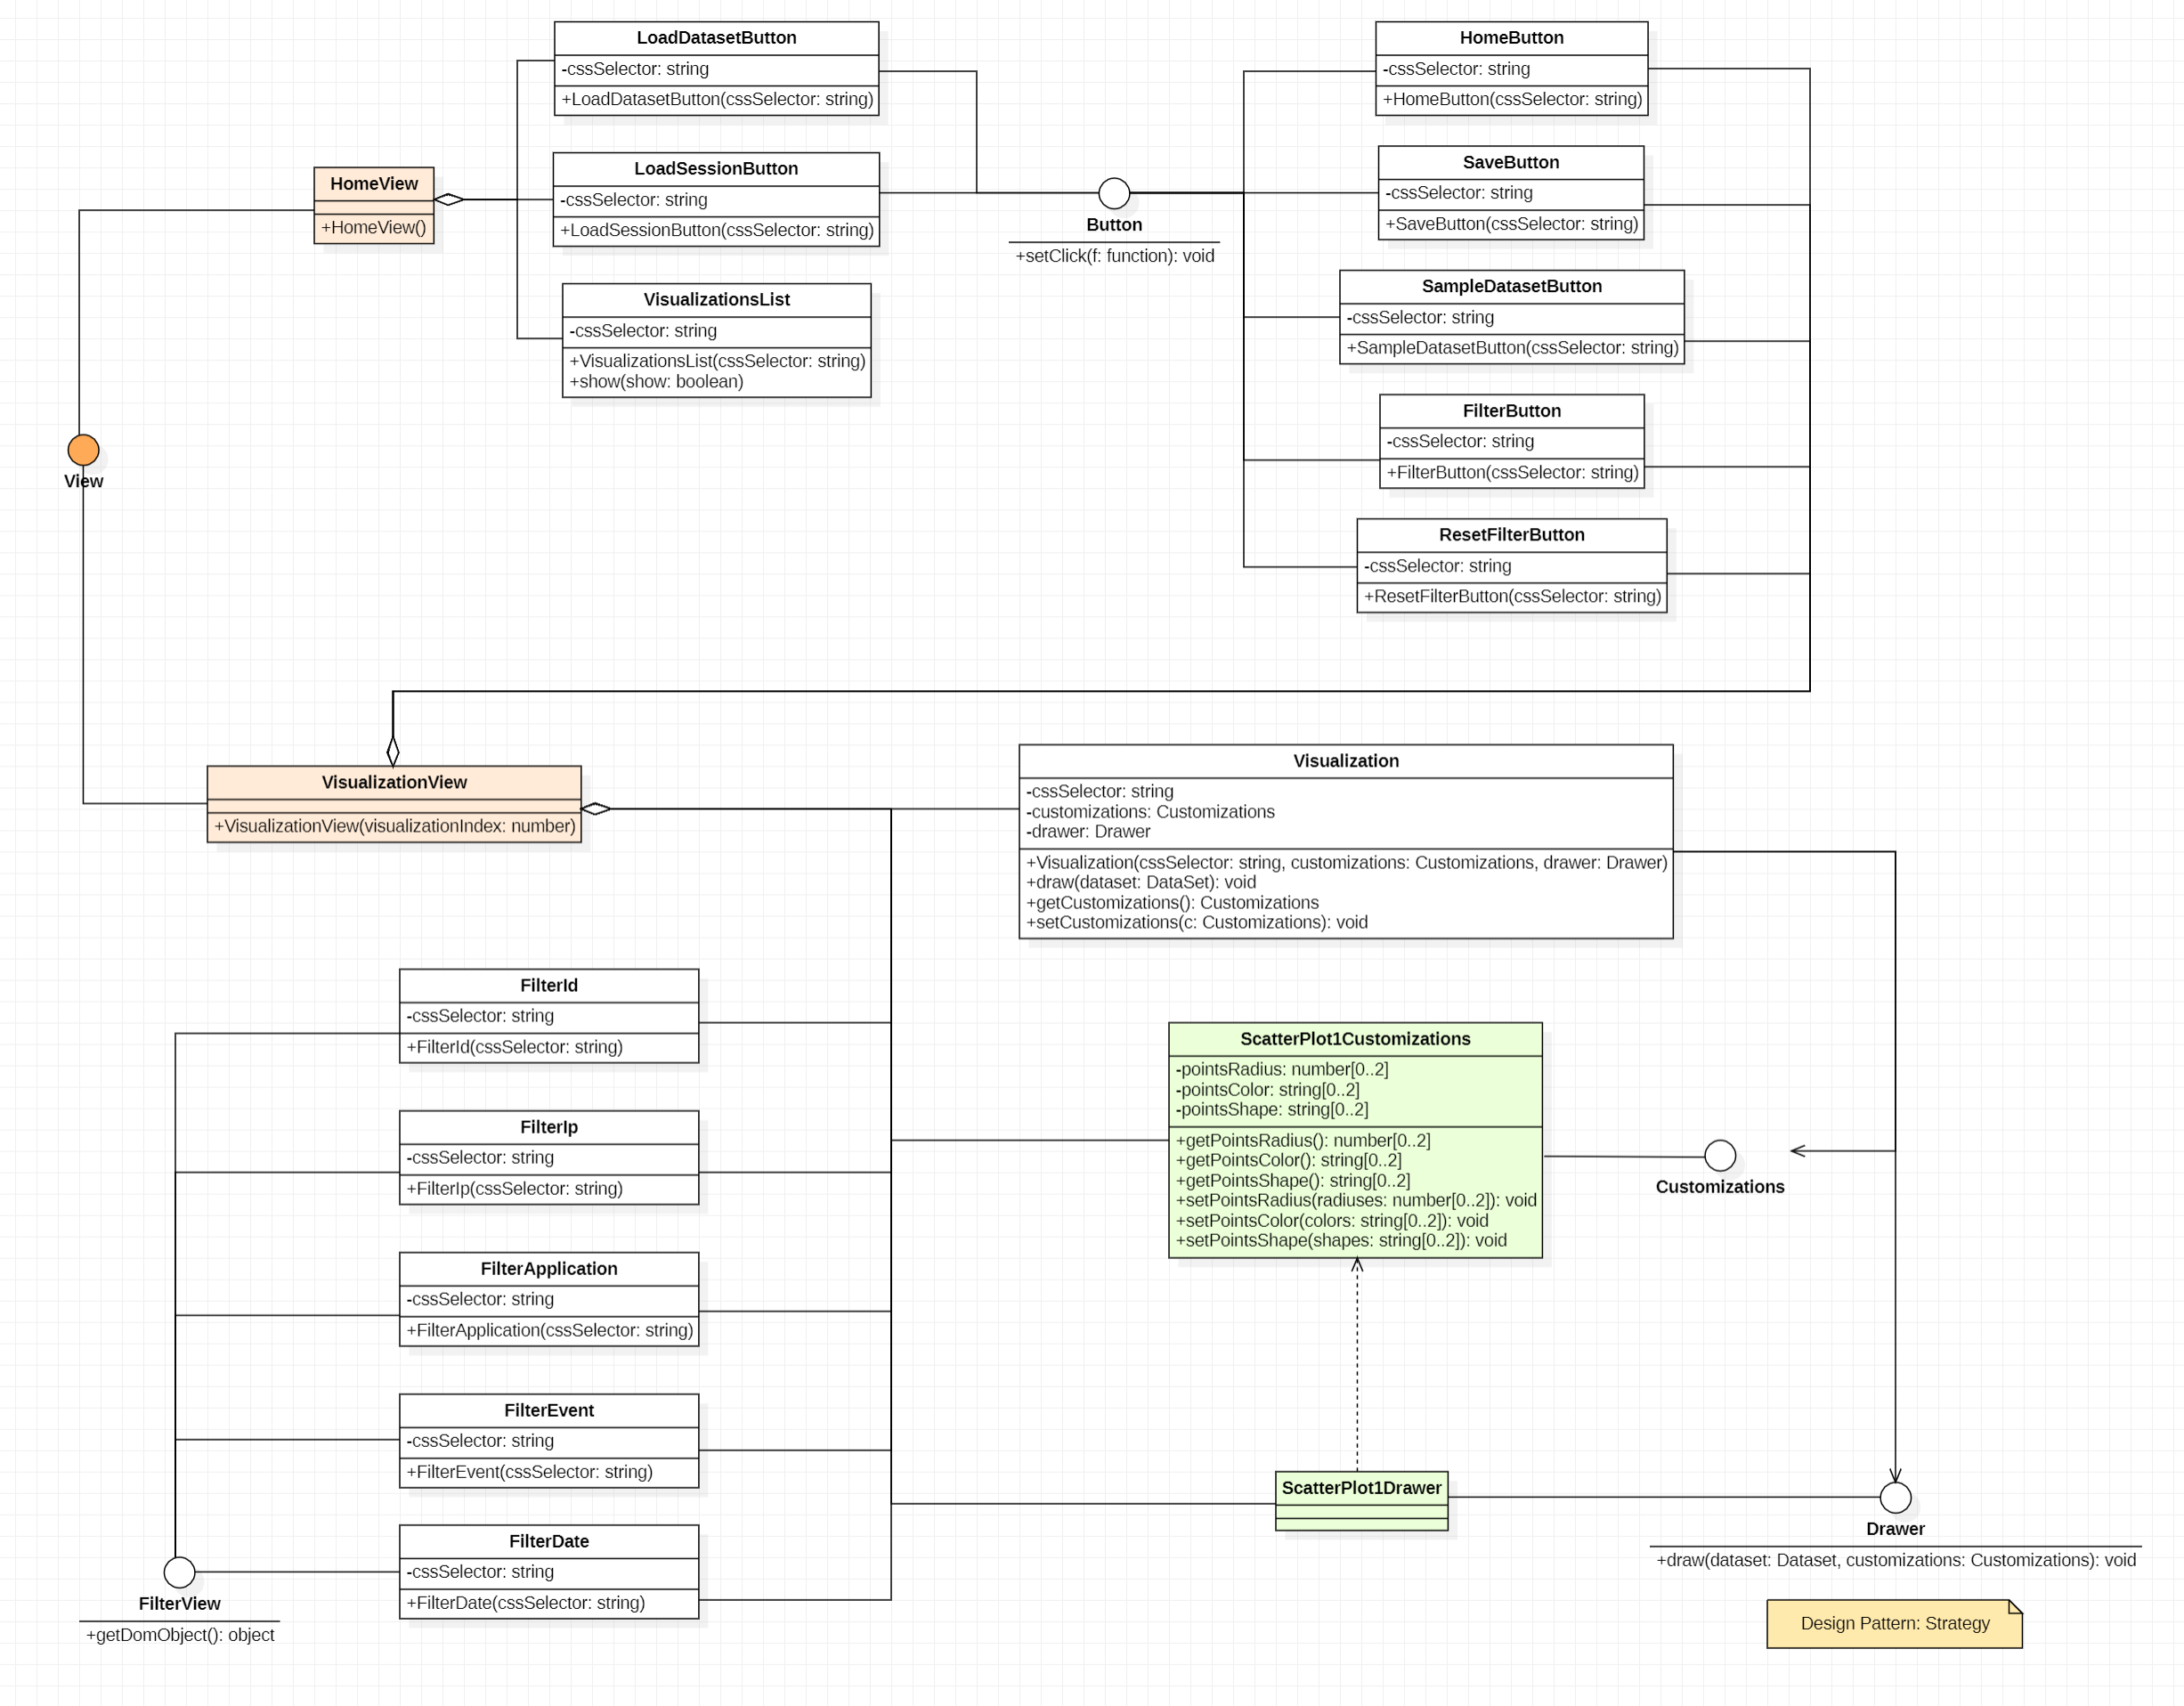
\includegraphics[width=1.0\textwidth]{vista.png}
    \caption{Diagramma delle classi riguardanti la vista}
\end{figure}
Il diagramma delle classi della vista è diviso principalmente in due parti: la classe \texttt{HomeView} e \texttt{VisualizationView} che si occupano di creare tutti gli elementi che compongono le rispettive viste e implementano un'interfaccia comune \texttt{View}.

Nella parte superiore del grafico si può notare che tutti i bottoni presenti nell'applicazione implementano l'interfaccia \texttt{Button} che mette a disposizione il metodo \texttt{setClick(f: function)} il quale conterrà l'event listener che verrà ridefinito da ogni bottone in base al suo compito.

In basso a sinistra si vede che i vari filtri impostabili implementano l'interfaccia \texttt{FilterView} che mette a disposizione il metodo \texttt{getDomObject()} il quale semplicemente restituisce l'elemento della DOM$_G$.

Come detto prima, la classe \texttt{VisualizationView} crea la classe \texttt{Visualization}, che si occupa di generare il grafico selezionato nella schermata home tramite il metodo \texttt{draw(dataset: Dataset)}, essa inoltre contiene i metodi che gestiscono le personalizzazioni dei grafici: \texttt{getCustomizations()} e \texttt{setCustomizations(c: Customizaions)}. \\Questa classe ha un riferimento alle interfacce \texttt{Drawer} e \texttt{Customizations}, dalle quali viene implementata una classe per ognuna possibile visualizzazione. In questo diagramma vengono inserite solo le classi Drawer e Customizations relative alla visualizzazione dello Scatter Plot numero 1 per renderlo più leggibile, ma come detto ogni visualizzazione ha le sue.
\subsection{Controller}
\section{Diagrammi di sequenza}
\subsection{Caricamento dataset}
\subsection{Nuovo campionamento}
\begin{figure}[H]
    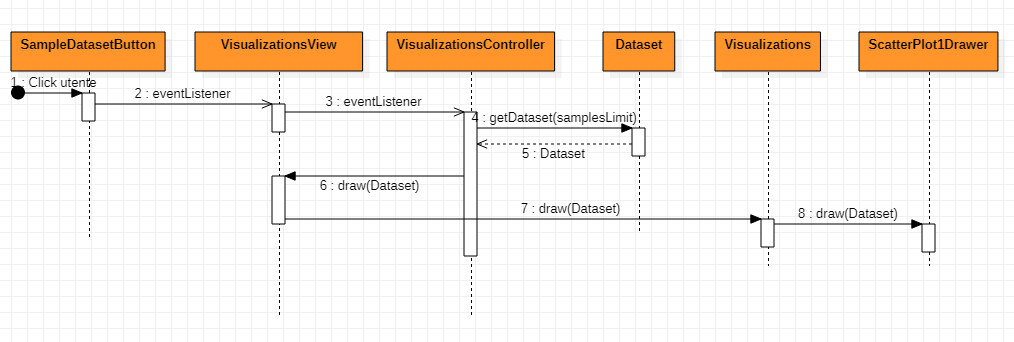
\includegraphics[width=1.0\textwidth]{sequenza_sample.png}
    \caption{Diagramma di sequenza per nuovo campionamento nel grafico \textit{ScatterPlot01}}
\end{figure}
\section{Design pattern utilizzati}
\subsection{Strategy}
\subsection{Template method}
Il gruppo ha deciso di utilizzare il \textit{Template Method} come design pattern comportamentale nel \textit{Controller}. \\Il motivo è che i due controller implementano un algoritmo \texttt{setup()} che ha un flusso di esecuzione comune ad entrambi: in ordine vengono eseguiti \texttt{setupStorage()}, \texttt{setupModel()} e \texttt{setupView()} che rispettivamente si occupano di creare il database, il modello e la vista. \\Ovviamente questi metodi avranno un comportamento diverso a seconda del controller in cui si trovano, ad esempio in \texttt{HomeController} il modello viene impostato dopo che l'utente ha caricato un file mentre in \texttt{VisualizationsController} il modello viene preso dal database del browser.
